Some underlying principles of the theoretical topics on which the  for this thesis are presented in this chapter.
All the topics of this chapter are present in the proposed model but some of the material is presented in greater detail that is completely necessary for understanding the model.

Firstly this chapter begins on the principles and handling of spatio-temporal data with emphasis on modelling it with advection fields.
Subsequently, an introduction to the neural network basics is presented.
Then the concepts of Bayesian filtering are presented and the Kalman filter defined with challenges and remedies related to the filtering of high-dimensional data. 

By reviewing these concepts, this chapter aims to give a foundation to understand the proposed model's underlying mechanisms presented in subsequent chapters

\subsection{Spatio-temporal Data}
The analysis of spatio-temporal data is an important part of research across many disciplines.
Spatio-temporal data is characterised by having both spatial, and temporal components that carry information across space, and over time.
Modelling these datasets requires thus observing and understanding how the phenomenon of interests evolves over time in many locations.
This subsection covers some basic principles of spatio-temporal data and dynamic modelling such data through the advection equation. 

\subsubsection{Defining Spatio-Temporal Data}
As to dismiss the Einstenian physics where space and time is interdependent, the classical way of separating the real spatial and temporal dimensions shall be considered here.

So now the spatial domain $\Omega$ is assumed to be a subset of $n$-dimensional real space, $\Omega \subset \R^n$, and the temporal domain $I$ a subset of the real line, $I \subset \R^1$.
Then the spatio-temporal domain is the Cartesian product of the spatial and temporal domains, $\Omega \times I$ and then an arbitrary spatio-temporal process can be written as
\begin{equation}
    \left\{ Y(x, t) \, \middle\vert \, x \in \Omega, \, t \in I \right\}.
\end{equation}

This way the spatio-temporal data may be thought as snapshots of some process at a specific point in time.
Naturally either, or both, the spatial and temporal variables may also be discrete by the nature of the quantities or due to discrete measurements.

A concrete example of spatio-temporal data could be air pollution data that tracks the concentration of pollutants accross different areas in a city and how it evolves over time.

\subsubsection{Dynamic Modelling of Spatio-Temporal Data}\label{subsubsection:dynamicmodellingspatiotemporaldata}
Dynamical modelling of spatio-temporal data refers to creating mathematical and computational models that explain changes of the observed variables in time.
Often some prior scientific information of the process is used to motivate the model.
This information is usually described with some partial differential equations (PDE).
At the core of the model of this thesis is the advection-diffusion equation describing the transportation and diffusion of the observed variable along some advection field in time.
In the air pollution example, the pollutants would be advected by winds, and diffused outwards of high concentrations.
A simplified example of data evolving through the advection-diffusion process is in Figure~\ref{fig:advection_diffusion}.

\begin{figure}[h]
    \centering
    \inputpypgf{background/fig/advectiondiffusion.pypgf}
    \caption{\label{fig:advection_diffusion}An example the of advection-diffusion process with two gaussian kernels.}
\end{figure}

The advection-diffusion equation consist of an advection part that describes the transportation, and diffusion that describes the diffusion process.
Consider a spatio-temporal function $u: \Omega \times I \rightarrow \R$ representing some quantity on spatial domain $\Omega \subset \R^n$, and temporal domain $I = (0, T)$.
The plain advection part is defined as
\begin{equation}\label{eq:advection}
    \frac{\partial u}{\partial t} =  - \mathbf{F} \nabla u,
\end{equation}
where $\mathbf{F} = \mathbf{F}(x,t)$ is the vector-valued advection field that transport $u$ forward in time.

Then the diffusion equation is
\begin{equation}\label{eq:diffusion}
    \frac{\partial u}{\partial t} = \nabla \cdot (D \nabla u),
\end{equation}
with $D = D(x,t)$ being the diffusion coefficient.
In many practical uses $D$ is assumed to be constant in space, and then the diffusion term $\nabla \cdot (D \nabla u)$ simplifies to $D \Delta u$ and diffusion equation~\eqref{eq:diffusion} recovers to the heat equation.

Now by combining~\eqref{eq:advection} and~\eqref{eq:diffusion} gives the advection-diffusion equation
\begin{equation}\label{eq:advectiondiffusion}
    \frac{\partial u}{\partial t} = \nabla \cdot (D \nabla u) - \mathbf{F} \nabla u.
\end{equation}

If the advection field $\mathbf{F}$, and the diffusion coefficient $D$ were known, and the model was perfect $u$ could be solved given some initial condition $u(\cdot, 0) = u_0(\cdot)$, and a boundary condition for the values of $u$ in the Dirichlet type case or the normal derivative of $u$ along the boundary of $\Omega$ in the Neumann type case.
However, measuring advection and diffusion parameters is often not possible and estimates $\overline{\mathbf{F}}$ and $\overline{D}$ need to be extracted e.g.\ from data.
While many uncertainties are involved in the parameter estimation, the model~\eqref{eq:advectiondiffusion} is also not a perfect representation so the approximate model
\begin{equation}\label{eq:advectiondiffusion_approx}
    \frac{\partial u}{\partial t} = \nabla \cdot (\overline{D} \nabla u) - \overline{\mathbf{F}} \nabla u + e
\end{equation}
needs to be considered where $e = e(x,t)$ is the (hopefully small) modeling error.
When taking real measurements, the model also needs to be discretised both in time so that each time step represents one measurement point, and in space so that $\Omega$ becomes a grid in which the measurements are taken at some resolution.

In the air pollution example the motivation for computing the estimates $\overline{\mathbf{F}}$ and $\overline{D}$ would be that assuming the real parameters change little in time, i.e.\ $\mathbf{F}(x,t_{k}) \approx \mathbf{F}(x,t_{k+1})$ and $D(x,t_{k}) \approx D(x,t_{k+1})$, the parameters can be utilised to transport air pollution images $u$ to to future and thus producing forecasts.

\subsection{Neural Networks}
Artificial neural networks drawing inspiration from the neural structures found in the human brain are a prominent part of modern machine learning methods.
With the dramatic increase in computing capabilities, more complex neural networks have became feasible for a variety of applications.
Substantial success in using neural networks has been found in various domains such as image classification, speech and text recognition, object detection, and automation of diverse tasks.

Over the decades of evolution since their inception in the 1940s as a mathematical model for nervous activity~\cite{mcculloch, hebb}, neural networks have undergone many transformations in terms of their architectures and capabilities.
In the 1950s to 1970s the first concepts were modelled with a single neuron but the application of backpropagation enabled optimising multiple layers of neurons laying foundations for the modern research of neural networks.
The most recent wave of neural networks research from the 2000's was spurred by powerful parallel computing performance that has enabled training of networks capable of learning increasingly complex phenomena.

In this thesis neural networks are employed as a tool to estimate advection fields from spatio-temporal data.
Given the nonlinear and dynamic nature of the underlying process, the task is inherently complex.
Nevertheless, eural networks provide a flexible framework for modelling these dynamics.

In the following parts basics of neural networks are covered starting from the McCulloch-Pitts Neuron and training it to backpropagation to the modern convolutional neural networks, which are central to this thesis.

\subsubsection{Neurons and Activation Functions}
The first mathematical model for neuron from~\cite{mcculloch}, known as the McCulloch-Pitts Neuron is the fundamental building block for any neural networks.
It consists of two principal components: an aggregation unit that processes the input vector, and an activation function that generates an output based on this aggregation.
The operational structure of the McCulloch-Pitts Neuron is illustrated in figure~\ref{fig:mccullochpittsneuron}.
\begin{figure}\label{fig:mccullochpittsneuron}
    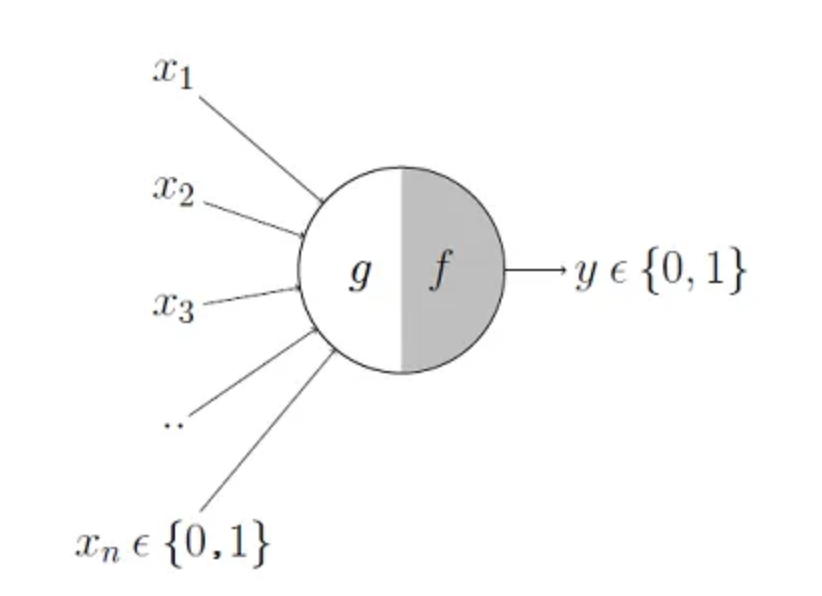
\includegraphics{background/fig/mccullochpitts.png}
    \caption{McCulloch-Pitts neuron (placeholder image)}
\end{figure}
The McCulloch-Pitts Neuron operates by taking an $n$-dimensional binary input vector $\mathbf{x}$ and applies function $f : \R^n \rightarrow \R$ that computes the sum of the inputs
\begin{equation}
    f(\mathbf{x}) = \sum_{i=1}^{n} x_{i}.
\end{equation}

The activation function $\phi$ subsequently determines the neuron's output based on a threshold $T$,
\begin{align}
    y = \phi(f(\mathbf{x})) & = 1 \text{ if } \phi(\mathbf{x}) \geq T \\
                            & = 0 \text{ if } \phi(\mathbf{x}) < T. 
\end{align}

While this is an attractive model in its simplicity, it has a major limitation.
Only binary input vectors $\mathbf{x}$ are accepted, and the output is always binary.

A few years later Donald Hebb~\cite{hebb} proposed that the proximity between inputs and other neurons should influence the output as well.
This concept was applied to the neuron model by Frank Rosenblatt~\cite{rosenblatt} who developed the much more flexible perceptron model.
Now the inputs can be any values, and they are weighted with a weight vector $\bm{w}$.
There is also a bias term in $f$.
Thus, the function $f : \R^n \rightarrow \R$ becomes
\begin{equation}
    f(\mathbf{x}) = \sum_{i=1}^{n} w_{i} x_{i} + b.
\end{equation}
The structure of the perceptron is depicted in figure~\ref{fig:perceptron}.

\begin{figure}\label{fig:perceptron}
    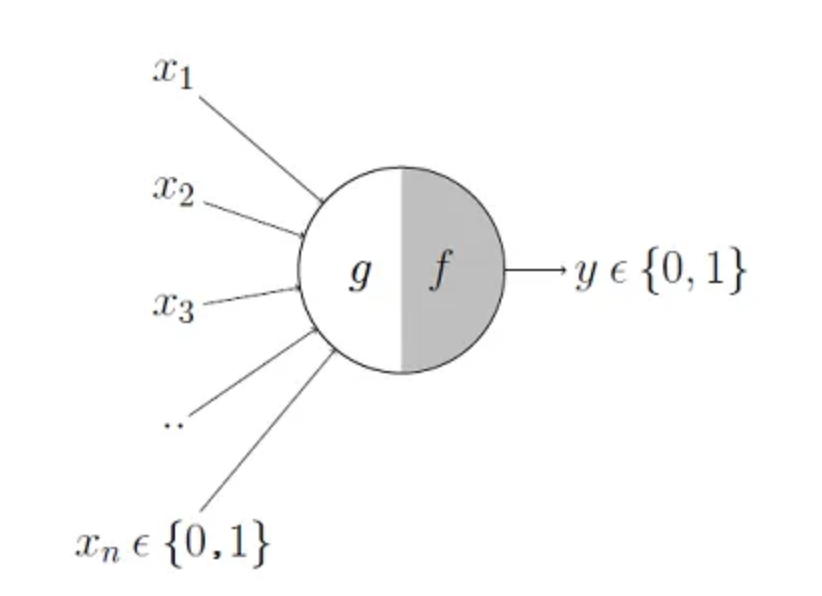
\includegraphics{background/fig/mccullochpitts.png}
    \caption{Perceptron (placeholder image)}
\end{figure}

The activation function $\phi$ can also be refined to be a more sophisticated one than just the binary step function.
Commonly used activation functions include the Rectified Linear Unit (ReLU) and the Leaky ReLU, the Sigmoid function, and the Softmax function.
The mentioned activation functions are visualised in figure~\ref{fig:activations}.
The choice of activation function comes with technicalities that are crucial for training a neural networks including the range of possible values and behavior of their derivatives.

\begin{figure}\label{fig:activations}
    \inputpypgf{background/fig/activations.pypgf}
    \caption{Different commonly used activation functions.}
\end{figure}

The single neuron model is only applicable to extremely simple tasks.
Therefore, the neurons were started to be arranged into layers to form a structure called Multilayer Perceptron (MLP).
The MLP is nothing more than combining a number of neurons in layers and applying them sequentially as shown in figure~\ref{fig:mlp}.
\begin{figure}\label{fig:mlp}
    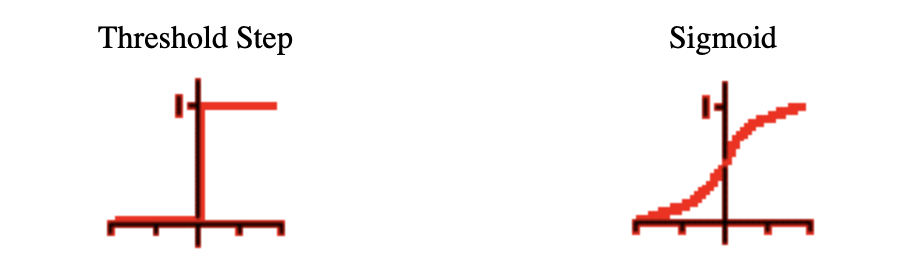
\includegraphics{background/fig/activations.png}
    \caption{Multilayer Perceptron (placeholder image)}
\end{figure}

Formally the MLP function $f^{(l)} : \R^n \rightarrow \R^m$ for layer $l$ is now
\begin{equation}
    f^{(l)}(\bm{x}; \bm{W}, \bm{b}) = \bm{W} \bm{x} + \bm{b},
\end{equation}
where rows of the weight matrix $\bm{W} \in \R^{n \times m}$ contain now the weights and the bias vector $\bm{b} \in \R^{m}$ has the bias terms of the neurons in the layer.
The activation function is now applied elementwise for the outputs of $f^{(l)}$.
And now the entire neural network is then a composition of all the layers.

MLPs are related to the important Universal Approximation Theorem presented at the turn of the 1990's.~\cite{cybenko,horniketal,hornik}
This theorem states that an MLP network with at least one hidden layer and any squashing activation function can approximate any Borel measurable function between finite-dimensional spaces.
While the theorem might sound compelling, the the number of neurons is not necessarily bounded for all functions even though there are some boundedness results for some classes of functions.
Therefore, this may lead to unfeasibly large networks.
Furthermore, the theorem does not state that any suitable function can be learnt, only that is can be represented.

While an MLP connects all the neurons in its layers, other types of neural networks such as convolutional ones, which are of primary interest in this work, allow partial connections between neurons creating a partially connected network.

\subsubsection{Convolutional Neural Networks}
Convolutional Neural Networks (CNNs) have emerged as an instrumental class of models garnering particular attention for their performance in tasks involving image data, e.g.\ image classification.
Their convolutional structure enables them to effectively identify the critical features and structures from spatial data.
While the fundamental concept is similar to that of the MLP model, CNNs are considerably distinct in their operation mechanics.
To better comprehend the working of the model used in this thesis, the specifics of CNNs are thus presented here in detail.

The convolution operation is the fundamental building block of CNNs.
The $n$-dimensional convolution of two compactly supported functions $f, g : \R^n \rightarrow \R$ is defined by
\begin{equation}
    (f * g)(x) = \int_{\R^n} f(y) g(x-y) \, \mathrm{d}y.
\end{equation}

In the context of neural networks, numerical operations need to be discretised.
So the discrete convolution for compactly supported $f, g : \Z^n \rightarrow \R$ is given by 
\begin{equation}
    (f * g)(x) = \sum_{y \in \N^{n}} f(y) g(x-y).
\end{equation}

In practical applications the dimension of the convolution seldom exceeds 4.
Particularly in the case of image data, two-dimensional convolutions are used and thus the examples from here on concern only the two-dimensional case.
Even though with a simple change of variables it is easy to see that the convolution is commutative, in neural networks $f$ is usually treated as some input data and $g$ as a convolution kernel.
However, practical neural network libraries implement a similar cross-correlation function~\cite{goodfellow}
\begin{equation}
    (f * g)(x) = \sum_{y \in \N^{n}} f(x) g(y+x),
\end{equation}
in which the kernel is not flipped, resulting in loss of the commutative property.
Nevertheless, this technicality does not affect the end result as the convolution kernel can be flipped to yield the same outcome.
Hence, these layers are referred as convolution layers, despite technically implemented as cross-correlations.

CNNs employ many small convolutions as a replacement for the dot product neurons found in the MLP layers.
With image inputs, the convolution kernels have often sizes of $3 \times 3$ or $9 \times 9$.
The smaller kernels are usually preferred  due to reduces model parameters and computational cost while still retaining the capacity of learning patterns from data.
The input is convoluted with a large number of these small kernels individually, and thus increasing the depth of the input.
A typical number of convolution filters in the initial layer could be 32 or 64, with increasing the number of filters when going deeper to the network to allow the model to learn more complex representations.
The idea is depicted in figure~\ref{fig:2dconv}.
\begin{figure}\label{fig:2dconv}
    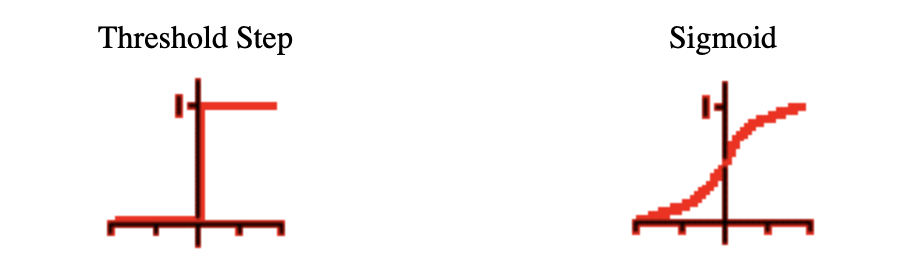
\includegraphics{background/fig/activations.png}
    \caption{2d convolution (placeholder image)}
\end{figure}

CNNs typically employ pooling layers for downsampling the spatial dimensions of the input by combining multiple values into one, usually by taking the average (average pooling) or maximum (max pooling) values.
Additionally, activation functions are applied after convolution layers along with some normalisations for the data in preparation of the next layer.
Convolutions with pooling and normalisations are rarely the sole type of layers in CNN architectures, and typically at least the very last layers are similar to the fully connected dot-product layers found in the MLP\@
These output layers are primarily for final classification and shaping the output of the network.

\subsubsection{Optimising Neural Network Parameters}
Computing a large number of the introduced numerical operations with arbitrary parameters have little use in practise.
Therefore a neural network has to unergo a training process during which the parametrs are optimised over a large training dataset.

Classically these learning tasks are divided into three categories: supervised, unsupervised, and reinforcment learning.
In supervised learning, data is labelled and the model learns by comparing it's output to the correct label.
Conversely, in unsupervised learning the model has to learn patterns in data without given labels.
Combinations of supervised and unsupervised learning also exist, called semi-supervised learning.
An example would be various forms of clustering tasks.
In reinforcment learning a model is trained to take some actions based on reward feedback and it learns to perform actions that maximise the cumulative reward. 

All these learning tasks with neural networks ultimately come down to an optimisation problem.
Optimising neural network parameters bears resemblance to other numerical optimisation methods, but due to the huge number of parameters and non-convex nature of the optimisation problems, training a neural network is a lengthy and complex task.
The optimisation problem of a supervised learning task can be written out as a minimisation of a real-valued cost functional $J$, which represents the expected value of a loss function, with respect to the network parameters $\bm{\theta}$:
\begin{equation}
    \min_{\bm{\theta}} \, J(\bm{\theta}) = \mathbb{E}_{(\bm{x},y) \sim \hat{p}_{\text{data}}} L(f(\bm{x}; \bm{\theta}), y) = \frac{1}{n} \sum_{i=1}^{n}  L(f(\bm{x}^{(i)}; \bm{\theta}), y^{(i)}).
\end{equation}
Here, $f$ denotes the neural network function that generates predictions given some input data $\bm{x}$, drawn from the empirical training data distribution, and the network parameters.
$L$ is the loss function comparing the network prediction, and the true label $y$.
This is easily modified to unsupervised learning by simply excluding $y$ from the equation in which case the loss function has to use some other method to compare correctness instead.

Choosing an appropriate loss function is a crucial part of model training.
The family of loss functions suitable for neural networks is large and dependent of the type of data.
While the definitions of different loss functions look very different, typically the choice is made based on how much large prediction errors should be compared to small errors.
Perhaps the most commonly used and well-known loss function is the mean squared error (MSE), which computes the mean of squared prediction errors:
\begin{equation}
    L_{\text{MSE}}(Y, \hat{Y}) = \frac{1}{n} \sum_{i=1}^{n} \left( Y_{i} - \hat{Y}_{i} \right)^{2}.
\end{equation}
In this equation, $Y$ represents the target value, and $\hat{Y}$ the predicted value.

Many optimisation algorithms with neural networks are, or are based on the Stochastic gradient descent (SGD).
SGD, an adaptation of the classic gradient descent algorithm, functions by adjusting the decision variable in the direction of the loss function's gradient, scaled by a small constant called the step size, or learning rate.
The stochastic version primarily differs from the original one by estimating gradients from a subset of the data, thereby reducing the computational cost.

With actual neural networks computing gradients of the objective function for the entire training dataset is not feasible, necessitating the computation of gradients from small samples of the training data.
For a true stochastic optimisation method only one sample would be taken but it is often more practical to take a small number of sampled and this is called minibatching.
The SGD algorithm with minibatching is laid out in detail in Algorithm~\ref{alg:sgd}.

\begin{algorithm}[H]
    \caption{Stochastic gradient descent}
    \label{alg:sgd}
    \begin{algorithmic}[1]
        \State\textbf{initialise} step size $\eta > 0$, initial parameter $\bm{\theta}$
        \While{stopping criterion not met} \Comment{E.g.\ non-decreasing losses}
        \State Sample a minibatch from training dataset $\{ (\bm{x}^{(i)}, y^{(i)}) \}_{i=1}^{m}$
        \State $\bm{d} = -\frac{1}{m} \nabla_{\bm{\theta}} \sum_{i=1}^{m} L(f(\bm{x}^{(i)}; \bm{\theta}), y^{(i)})$ \Comment{Compute search direction}
        \State $\bm{\theta} = \bm{\theta} + \eta \bm{d}$ \Comment{Update parameters}
        \EndWhile
        \State\textbf{return} $\bm{\theta}$
    \end{algorithmic}
\end{algorithm}

The stochastic nature of the SGD algorithm introduces some noise into the computes losses.
As a result, the step size needs to be decreased in training at some rate to mitigate the issue as that noise occurs also in the optimum.
Many techniques exist for step size scheduling and while used utilised in training the model of this thesis but this is mostly a technical detail and outside the scope of this section.
For those interested in exploring further,~\cite{goodfellow} provides some in-depth discussions on the subject.

More sophisticated optimisation algorithms are also often employed in optimising neural networks.
SGD with momentum, for instance, supplements the current search direction with a fraction of the previous one robostify the search directions.
Some other popular optimisation algorithms used for neural network training include RMSProp, AdaDelta, and Adam, with the latter combining the benefits of RMSProp and AdaGrad.
Again,~\cite{goodfellow} provides detailed explanations of many other algorithms.

The different algorithms have each offer distinct advantages, for example some don't have the issue of scheduling step sizes as with SGD, but there is no universal algorithm that would be best for all cases.
However, the common theme is the iterative update of the model parameters by moving in the direction of the gradient of the loss function.
Hence the next challange is then to efficiently compute these gradients.

\subsubsection{Backpropagation}
Training a neural network starts with computing predictions of the network using some inputs from training dataset.
This part if often called forward propagation.
However, in all optimisation algorithms at some point the gradient of a scalar loss function is needed.
This part is called backpropagation.
Numerically computing gradients in the conventional way for neural networks consisting a huge number of parameters is computationally infeasible, and thus some other methods are required to train a network in practise.

Reverse accumulation as an automatic differentiation technique for MLP networks was first introduced in the 1970's and 1980's, later became known as backpropagation.
Backpropagation was first introduced by Paul Werbos in their 1974 PhD thesis~\cite{werbos}, but gained popularity a decade later through the works of David Rumelhart and others~\cite{rumelhartetal}.

These works facilitated the efficient training of more complex networks due to the precise gradient estimation of neural network parameters.
However, reverse accumulating gradients was studied independently by multiple others even earlier.
Perhaps the most notable example being the works of the Finnish mathematician Seppo Linnainmaa in their MSc thesis from 1970~\cite{linnainmaa}.
Although then the concept of reverse accumulation was studied in cumulative floating point errors.

The core principle behind the backpropagation algorithm is the recursive application of the chain rule of calculus.
The chain rule states that for $g: \R^{m}\rightarrow \R^{n}$ and $f: \R^{n} \rightarrow \R$ with $f(g(\bm{x}))$ the partial derivatives of $f$ are given by
\begin{equation}
    \frac{\partial f}{\partial \bm{x}_{i}} = \sum_{j = 1}^{n} \frac{\partial f}{\partial (g(\bm{x})_{j})} \frac{\partial (g(\bm{x})_{j})}{\partial x_{i}}.
\end{equation}

The objective function $J$ of the optimisation problem can be considered as a composition of all the individual functions in the network.
Subsequently, the chain rule can be used to obtain the partial derivatives with respect to the trainable network parameters.

As the shapes and sizes of the trainable parameters may be different for each specific network architecture, the exact formulation of the gradients might differ a bit.
For the simple MLP case the formulas are easy to write to see what is the idea behind the backpropagation algorithm.
Recall that the network parameters can be expressed for each layer $\ell$ as a matrix $\bm{\theta}^{(\ell)} = \begin{bmatrix} \bm{W} & \bm{b} \end{bmatrix}^{(\ell)}$. Then mark the output of layer $\ell$ as $\bm{z}^{(\ell)} = \bm{W}^{(\ell)} \bm{a}^{(\ell-1)} + \bm{b}$ where $\bm{a}^{(\ell-1)} =  \phi^{\ell-1}(\bm{z}^{(\ell-1)})$ is the output from the activation of the previous layer.
Now the chain rule thus gives the
\begin{equation}\label{eq:mlpchainrule}
    \frac{\partial J}{\partial \bm{\theta}_{ij}^{(\ell)}} = \sum_{k} \frac{\partial J}{\partial \bm{z}_{k}^{(\ell)}} \frac{\partial \bm{z}_{k}^{(\ell)}}{\partial \bm{\theta}_{ij}^{(\ell)}}. 
\end{equation}
Now the $\bm{z}$ derivatives are easily evaluated for the weight terms to
\begin{equation}
    \frac{\partial J}{\partial \bm{W}_{ij}^{(\ell)}} = \frac{\partial J}{\partial \bm{z}_{j}^{(\ell)}} \bm{z}_{i}^{(\ell)},
\end{equation}
and for the bias terms to
\begin{equation}
    \frac{\partial J}{\partial \bm{b}_{j}^{(\ell)}} = \frac{\partial J}{\partial \bm{z}_{j}^{(\ell)}} 1.
\end{equation}
Thus~\eqref{eq:mlpchainrule} can now be written as
\begin{equation}\label{eq:mlchainrulevec}
    \bm{\nabla}_{\bm{\theta}^{(\ell)}} J = \begin{bmatrix} \bm{x}^{(\ell)} \\ 1 \end{bmatrix} (\nabla_{\bm{z}^{(\ell)}} J)^{\top}.
\end{equation}
What is left now is to find an equation for the gradient term of~\eqref{eq:mlchainrulevec} that is often called the local gradient or error is usually denoted by $\bm{\delta}^{(\ell)}$.
By applying the chain rule once again,
\begin{align}
    \delta_{j}^{(\ell)} = \frac{\partial J}{\partial \bm{z}_{j}^{(\ell)}} = &\sum_{k} \underbrace{\frac{\partial J}{\partial \bm{z}_{k}^{(\ell + 1)}}}_{=\delta_{k}^{(\ell+1)}} \frac{\partial \bm{z}_{k}^{(\ell+1)}}{\partial \bm{z}_{j}^{(\ell)}} \\
                                                                       &= \sum_{k} \delta_{k}^{(\ell+1)} \frac{\partial \bm{z}_{k}^{(\ell+1)}}{\partial \bm{z}_{j}^{(\ell)}},
\end{align}
from which
\begin{align}
    \frac{\partial \bm{z}_{k}^{(\ell+1)}}{\partial \bm{z}_{j}^{(\ell)}}  = \frac{\partial}{\partial \bm{z}_{j}^{(\ell)}} \sum_{i} \bm{W}_{ki}^{(\ell+1)} \phi^{(\ell)}(\bm{z}_{i}^{(\ell)}) + \bm{b}_{k}^{(\ell+1)} = \bm{W}_{kj}^{(\ell+1)} \phi^{(\ell)\prime} (\bm{z}_{j}^{(\ell)}).
\end{align}
Thus for the error is now recursively
\begin{equation}
    \delta_{j}^{(\ell)} =  \sum_{k} \delta_{k}^{(\ell+1)} \bm{W}_{kj}^{(\ell+1)} \phi^{(\ell)\prime} (\bm{z}_{j}^{(\ell)}).
\end{equation}
For the last layer $L$ the error can be given more simply,
\begin{align}
    \delta_{j}^{(L)} = \frac{\partial J}{\partial \bm{z}_{j}^{(L)}} &= \sum_{k} \frac{\partial J}{\partial \bm{a}_{k}^{L}} \underbrace{\frac{\partial \bm{a}_{k}^{L}}{\partial \bm{z}_{j}^{L}}}_{=0\text{ when } k \neq j} \\
                                                                    &= \frac{\partial J}{\partial \bm{a}_{j}^{L}} \frac{\partial \bm{a}_{j}^{L}}{\partial \bm{z}_{j}^{L}}\\
                                                                    &= \frac{\partial J}{\partial \bm{a}_{j}^{L}} \phi^{(L)\prime} (\bm{z}_{j}^{(L)}).
\end{align}

Now that the neural network can be constructed, there is a way to find the optimal network parameters with computing easily the gradients, a complete neural network can be trained.
Typically most of these things presented are encapsulated inside the numerical neural network libraries the most-well known examples being PyTorch and Tensorflow.

\subsection{Bayesian Filtering}
Bayesian filtering refers to to the Bayesian way of deriving an optimal filtering problem of estimating the state of a nonstationary system through some observations.
This approach becomes valuable when dealing with real-world phenomena where a mathematical model can approximate the temporal evolution of some process and measurements of the system may be uncertain.


A key application of Bayesian filtering is state estimation which emerges in many disciplines.
It involves estimating a hidden state of a system based on some available indirect and noisy measurements.
Bayesian filtering provides a robust mathematical framework to combine prior knowledge about a system's state with new measurements to enhance state estimates over time.

The Bayesian filtering theory emerged at the turn of the 1960s with perhaps the most famous example being the works of Rudolf E. Kálmán who published a recursive solution to a linear special case of the problem in~\cite{kalman}.
Meanwhile in the Soviet Union Ruslan, Stratonovich studied the more general nonlinear Bayesian filtering problem, see e.g.~\cite{stratonovich2, stratonovich1}.
The simultaneous advances in digital computers allowed the theory to prove itself quickly useful in many applications, an early well-known example of which is the guidance system of the Apollo spacecraft~\cite{mcgee}.

In the context of this work, Bayesian filtering is employed to manage uncertainties related to the neural network model.
The neural network is capable of capturing the advection fields, and the Bayesian filtering framework provides a way to generate probailistic state estimates of the COT data.

\subsubsection{Bayesian Inference}
Bayesian inference refers to the process of updating prior probability estimates in light of more information.
The basis of Bayesian inference is the Bayes' Theorem.
\begin{theorem}[Bayes' Theorem]
    Assume a known prior probability density function $\pi(x)$ from a random variable $X$, and an observed probability $\pi(y)$ from another random variable $Y$.
    Then the posterior distribution of $X$ given the observed data is given by
    \begin{equation}
        \pi(x \, \vert \, y) = \frac{\pi(x) \pi(y \, \vert \, x)}{\pi(y)}.
    \end{equation}
\end{theorem}
In Bayesian inference, the prior distribution contains the information of some quantity before observing the data, and the posterior distribution the updated information after the observation.
Bayesian inference revolves around using data to transform the prior distributions into the posterior distributions.

\subsubsection{Probabilistic state-space models}
The Bayesian framework of assimilating measurements, using a process model, and producing forecasts from them can be formalised as the state-space model.
Given the inherent uncertainties linked with measurments and modelling, instead of focusing solely on point estimates of the state, it is substantially more fruitful to consider probability distributions.

Consider two stochastic processes, $\{X_k\}_{k=0}^{\infty}$ and $\{Y_k\}_{k=0}^{\infty}$, denoting the state and measurements of a system respectively.
Figure~\ref{fig:statespacedependency} presents the dependency scheme of the processes needed to formulate the state-space model.
\begin{figure}[h]
    \begin{alignat*}{5}
    \text{State:}& \quad && X_0 \, \rightarrow \, && X_1 \, \rightarrow \, && X_2 \,\rightarrow \cdots \rightarrow \, && X_k \, \rightarrow \cdots \\
                 & &&  && \downarrow && \downarrow && \downarrow \\
    \text{Observations:}& \quad && && Y_1 && Y_2 && Y_k
\end{alignat*}

    \caption{\label{fig:statespacedependency}Dependency scheme of the state-space model.}
\end{figure}
In order for the dependencies of the figure to materialise, some assumptions about the processes are required:
\begin{enumerate}
    \item 
        $\{X_k\}_{k=0}^{\infty}$ satisfies the Markov property with respect to its own history, and history of the observations:
        \begin{equation*}
            \pi (x_{k+1} \, \vert \, x_{0:k}, y_{1:k}) = \pi (x_{k+1} \, \vert \, x_k).
        \end{equation*}
    \item
        $\{Y_k\}_{k=0}^{\infty}$ satisfies the Markov property with respect to the history of the true state:
        \begin{equation*}
            \pi (y_k \, \vert \, x_{0:k}) = \pi (y_k \, \vert \, x_k).
        \end{equation*}
\end{enumerate}
With these assumptions the probabilistic state-space model can be defined.
\begin{definition}[Probabilstic state-space model]\label{def:state-space}
    Assume stochastic processes $\{X_k\}_{k=0}^{\infty}$ and $\{Y_k\}_{k=0}^{\infty}$ meet the previous assumptions.
    Then the following conditional probability distributions define the probabilstic state-space model:
    \begin{subequations}\label{eq:statespace}
        \begin{align}
            X_0 &\sim \pi (x_0)\\
            X_{k+1} &\sim \pi (x_{k+1} \, \vert \, x_{k}), \quad k = 0,1,2,\dots \label{eq:statespace1}\\
            Y_k &\sim \pi (y_k \, \vert \, x_k), \quad k = 1,2,\dots. \label{eq:statespace2}
        \end{align}
    \end{subequations}
\end{definition}
In Definition~\ref{def:state-space},~\eqref{eq:statespace1} is the model that describes the evolution of state over time, and~\eqref{eq:statespace2} is the observation model that describes the distribution of measurements conditioned on the state.

If functions for the state evolution and observations are known, the same can also be alternatively written as 
\begin{subequations}\label{eq:statespacemodel}
    \begin{align}
        X_{k+1} &= M_{k+1}(X_{k}, W_{k+1}), \quad k = 0,1,\dots \label{eq:statespacemodel1}\\
        Y_{k} &= H_{k}(X_{k}, V_{k}), \quad k = 1,2,\dots. \label{eq:statespacemodel2}
    \end{align}
\end{subequations}
Now~\eqref{eq:statespacemodel1} is the state evolution equation where function $M_{k+1}$ gives the next state $X_{k+1}$ given the previous state $X_{k}$ and the state noise $W_{k+1}$
The observation equation~\eqref{eq:statespacemodel2} describes the observations $Y_{k}$ as being the output of the observation function $H_{k}$ with the true state $X_{k}$ and the observation noise $V_{k}$.

For the probailistic state-space models, a few conditional probability distributions are usually of interest outlined in the following definition.
\begin{definition}
    Assume two stochastic processes $\{X_k\}_{k=0}^{\infty}$ and $\{Y_k\}_{k=0}^{\infty}$ form a probabilistic state-space model.
    Then the conditional probability distribution
    \begin{itemize}
        \item
            $\pi(x_k \, \vert \, y_{1:k})$ is a filtering distribution.
        \item
            $\pi(x_{k+n}\, \vert \, y_{1:k}), \, n > 0$ is a prediction distribution.
        \item
            $\pi(x_k \, \vert \, y_{1:})$ is a smoothing distribution.
    \end{itemize}
\end{definition}

With the state-space model~\eqref{eq:statespace} the Bayesian filtering problems can be discussed.
The idea behind Bayesian filtering is to recursively update the predictions and states of the model given latest observations.
The following theorem presents the two update equations for the Bayesian filtering scheme.
\begin{theorem}[Bayesian filtering equations]\label{thm:updateformulas}
    Let $\{X_k\}_{k=0}^{\infty}$ be a state process and $\{Y_k\}_{k=0}^{\infty}$ an observation process in a state-space model.
    Then the following recursive equations for Bayesian filtering steps apply:
    \begin{enumerate}
        \item 
            Prediction step:
            \begin{equation}\label{eq:predictionstep}
                \pi (x_{k+1} \, \vert \, y_{1:k}) = \int \pi (x_{k+1} \, \vert \, x_k) \pi (x_k \, \vert \, y_{1:k}) \, d x_k.
            \end{equation}
        \item
            Observation update step:
            \begin{equation}\label{eq:updatestep}
                \pi(x_{k+1} \, \vert \, y_{1:k+1}) = \frac{\pi (y_{k+1} \, \vert \, x_{k+1}) \pi (x_{k+1} | y_{1:k})}{\pi (y_{k+1} \, \vert \, y_{1:k})},
            \end{equation}
            with
            \begin{equation*}
                \pi (y_{k+1} \, \vert \, y_{1:k}) = \int \pi (y_k \, \vert \, x_k) \pi (x_k \, \vert \, y_{1:k-1}) \, d x_{k+1}.
            \end{equation*}
    \end{enumerate}
\end{theorem}
\begin{proof}
    In Appendix~\ref{app:proofs}.
\end{proof}

Theorem~\ref{thm:updateformulas} provides a framwork for efficiently computing probability distributions conditioned on observations.
The prediction step equation~\ref{eq:predictionstep} being the joint probability distribution of the current and next state conditioned on the latest observations facilitates probabilistic state estimates.
Then the observation update equation~\ref{eq:updatestep} is just the Bayes formula where $\pi (x_{k+1} \, \vert \, y_{1:k})$ is interpreted as the prior information of the state for statistical inversion of a new observation.

\subsubsection{Kalman Filter}
The Kalman filter provides an elegant closed-form solution for the update equations of Theorem~\ref{thm:updateformulas} in the special case of a linear state-space model with Gaussian additive noise process.
In this special case the state-space model corresponding to~\eqref{eq:statespacemodel} becomes
\begin{subequations}\label{eq:kalmanstatespace}
    \begin{align}
        X_{k+1} &= M_{k+1}X_{k}  + W_{k+1}, \quad W_{k+1} \sim \mathcal{N}(0, Q_{k+1})\\
        Y_{k} &= H_{k}X_{k} + V_{k}, \quad V_t \sim \mathcal{N}(0, R_k)
    \end{align}
\end{subequations}
with a Gaussian distribution for the initial state $X_0$.

Under these assumptions, the state's probability densities of the state of the model can be given by just estimates of the mean and covariance.
The following theorem gives the filtering step equations of Theorem~\ref{thm:updateformulas}.
\begin{theorem}[Kalman filter equations]\label{thm:kalmanfilterupdate}
    Assume a linear Gaussian state-space model~\eqref{eq:kalmanstatespace}.
    Let $x_{k\,\vert\,\ell}$ and $P_{k\,\vert\,\ell}$ represent the a posteriori mean and covariance of the state at time $k$ given observations $y_{1:\ell}$.
    Then the filterering equations of Theorem~\ref{thm:updateformulas} take closed form solutions:
    \begin{enumerate}
        \item 
            Prediction step:
            Given
            \begin{equation*}
                \pi (x_k \, \vert \, y_{1:k}) \sim \mathcal{N}(x_{k\,\vert\,k}, P_{k\,\vert\,k}),
            \end{equation*}
            a priori distribution of the next state is
            \begin{equation*}
                \pi (x_{k+1} \, \vert \,  y_{1:k}) \sim \mathcal{N}(\hat{x}_{k+1\,\vert\,k}, \hat{P}_{k+1\,\vert\,k}),
            \end{equation*}
            where parameters of the distribution are given by
            \begin{subequations}\label{eq:kalmanpredictionstep}
                \begin{align}
                    \hat{x}_{k+1\,\vert\,k} &= M_{k+1}x_{k\,\vert\,k}\\
                    \hat{P}_{k+1\,\vert\,k} &= M_{k+1}P_{k\,\vert\,k}M_{k+1}^{\top} + Q_{k+1}.
                \end{align}
            \end{subequations}
        \item
            Observation update step:
            Given
            \begin{equation*}
                \pi (x_{k+1} \, \vert \,  y_{1:k}) \sim \mathcal{N}(x_{k+1\,\vert\,k}, P_{k+1\,\vert\,k}),
            \end{equation*}
            a posteriori distribution of the next state is
            \begin{equation*}
                \pi (x_{k+1} \, \vert \,  y_{1:k+1}) \sim \mathcal{N}(x_{k+1\,\vert\,k+1}, P_{k+1\,\vert\,k+1}).
            \end{equation*}
            With 
            \begin{subequations}\label{eq:kalmanupdatestep}
                \begin{align}
                    v_{k+1} &= y_{k+1} - H_{k+1}x_{k+1 \, \vert \, k},\\
                    S_{k+1} &= H_{k+1} \hat{P}_{k+1\,\vert\,k} H_{k+1}^{\top},\\
                    K_{k+1} &= \hat{P}_{k+1\,\vert\,k}  H_{k+1}^{\top} S_{k+1}^{-1},\\
                    x_{k+1\,\vert\,k+1} &= \hat{x}_{k+1\,\vert\,k} + K_{k+1} v_{k+1},\\
                    P_{k+1\,\vert\,k+1} &= (I-K_{k+1}H_{k+1})\hat{P}_{k+1\,\vert\,k}.
                \end{align}
            \end{subequations}
    \end{enumerate}
\end{theorem}
\begin{proof}
    In Appendix~\ref{app:proofs}.
\end{proof}
While the theorem assumes zero means for noises, the Gaussian distributions can easiliy be shifted to accomodate for non-zero means, too.
The Kalman filter leverages the property of Gaussian distributions retaining their Gaussian form under affine transformations.
However, for nonlinear state-space models one can use linear approximations in order to preserve the convenience of Gaussian densities, a method known as extended Kalman filter.

Even when the assumptions for the Kalman filter apply, with larger states and observation spaces, problems will arise with computing the Kalman filter steps.
The matrix update formulas of Theorem~\ref{thm:kalmanfilterupdate} cross quickly the limits of computational feasibility.
One way of tackling the problem is to use Ensemble Kalman filters.

\subsubsection{Ensemble Kalman Filter}
Despite the effectiveness of the original Kalman filter in optimal filtering problems, it doesn't scale well with large state and observation spaces.
This limitation leads to the Ensemble Kalman Filter (EnKF).
It was first introduced by Geir Evensen in~\cite{evensen1994} as a Monte Carlo approach to the Kalman filter.
EnKF circumvents the large covariance matrices by representing a state of an state-space model by Monte Carlo samples from which sample covariances are computed.

